%Overskrifter er kokt, endre dem så det passer.

%Kommentarene nedenfor gjelder situasjoner og elementer fra gruppelogg som skal
%dras inn. I tillegg må det reflekteres, og relevant teori må dras inn
\chapter{Analyse av gruppearbeidet}

\section{Kompetanse i praksis}

Samtlige gruppemedlemmer følger sivilingeniørstudiet på NTNU, og har som en
konsekvens av det den samme faglige ``grunnpakken''. Dette har gjort det enklere
for gruppemedlemmene og kommunisere på tvers av fagfeltene, da alle behersker
basisterminologi innen f.eks. fysikk, matematikk, statistikk og data. Utover
dette har gruppemedlemmenes kompetanse fått praktisk utfoldelse gjennom det vi
godt kan kalle naturlig oppgavefordeling. Knut Halvor, med bakgrunn fra
datateknikk, har hatt hovedansvar for programmering. Fysikeren på gruppa,
Åsmund, har taklet differensialligningenes praktiske anvendelse, mens gapet
mellom programimplementasjon og fysisk problem har blitt fylt (les:
diskretisert) av Turid og Paul, matematikerene på gruppa. Joakim, som har
spesialisering innenfor konstruksjonsteknikk, har bidratt litt over det hele, da
han har generell kunnskap innen de samme fagfeltene. Gjennom tilbakemelding på
gruppelogger viste det seg også at Joakim var flink til å skrive prosess, slik
at han fikk tildelt endel ansvar med tanke på prosessrapport. \\

Det har i så måte vært meget tilfredstillende og se at teoretisk kunnskap kan
benyttes til å beskrive praktiske fysiske fenomener, og at overenstemmelsen
mellom numerisk simulering og eksperiment er god. \\ 

\emph{Jeg fant dette kapittelet tungt å skrive om, vi må ha mer her.. Plenum
plz?!}

%Føler denne kan inn her - Åsmund
Som et eksempel på kompetanse i praksis presenterer vi en grafisk fremstilling
av et utdrag av loggen på github, \cref{fig:github}.
\begin{figure}[h!]
  \begin{center}
    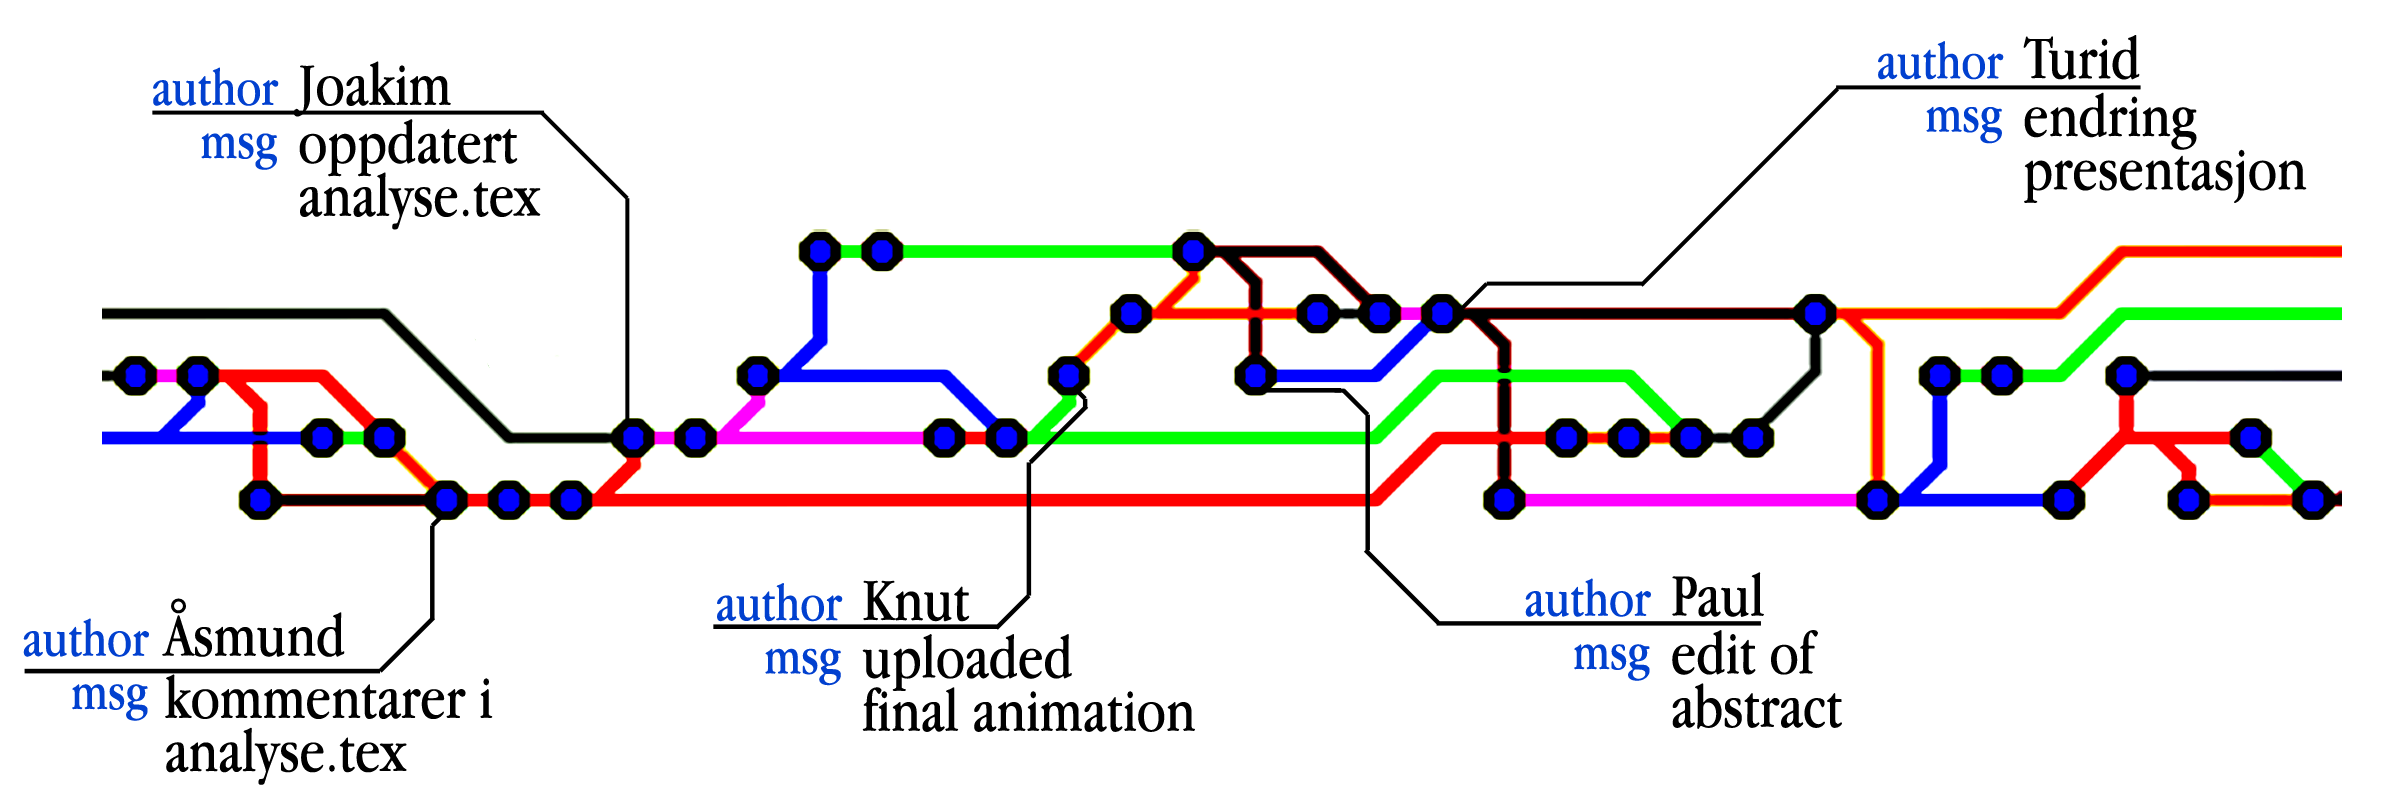
\includegraphics[width=\textwidth]{github.png}
  \end{center}
  \caption{Et utdrag fra commit-treet for arbeidet på github}
  \label{fig:github}
\end{figure}
Her ser man hvordan de forskjellige medlemmene både har arbeidet på forskjellige
deler av prosjektet, og hvordan man 

\section{Kommunikasjon og samspill}
Det kommunikasjonsnettverket som ble brukt på gruppa vår var åpent nettverk og sirkel nettverk. 
I et åpent nettverk kommuniserer alle med alle. Denne formen for kommunikasjon kommer tydelig fram 
i diskusjoner på gruppen der det er fri flyt av ideer og meninger. Når en avgjørelse blir tatt på 
gruppen starter vi ofte med en åpen diskusjon, og utvekslinger av meninger. Før en avgjørelse blir 
tatt har vi vanligvis hatt en runde rundt bordet der alle får uttrykt sin mening om saken. Dette er 
en form for sirkel nettverk, der et medlem uttrykker sin mening før han sender ordet videre til sidemannen.
 Dette er en kommunikasjonsform som har utviklet seg naturlig på gruppen. Særlig i prosessdelen har 
 det falt naturlig å ta en runde rundt bordet for å høre de ulike medlemmenes meninger og følelser. 
 Her er det ofte Turid som har tatt initiativ til runde rundt bordet, og har dermed falt inn i en 
 rolle som ordstyrer. Etterhvert som gruppen ble bedre kjent var det flere som gikk inn i rollen 
 som ordstyrer, når de følte det var nødvendig. Dette førte til at vi fikk en naturlig styringsprosess
  ved gruppediskusjoner, uten at vi trengte å skrive en formell regel i gruppekontrakten.\\

%%%%%%%%%%%%%%%%%%%%%%%%%%%%%%%%%%%%%%%%%%%%%%%%%%%%%%%%%%%%%%%%%%
Gruppelogg 11:
Etter lunsj var det en meget god gruppeaktivitet i regi læringsassistentene.
Gruppemedlemmene skulle ved hjelp av poeng, rangere seg selv og gruppemedlemmer
i ulike situasjoner. Vi hadde på forhånd bestemt oss for at presentasjonen av
gruppa i prosessrapporten skulle inneholde to aspekter pr. gruppemedlem.
\begin{itemize}
\item Gruppemedlemmets egen oppfatning av seg selv
\item Gruppas oppfatning av personen
\end{itemize}
Altså var denne biten av prosessrapporten en naturlig forlengelse av øvingen, og
dermed noe vi følte vi hadde stort utbytte av.

Verdt å kommentere er at gruppen (tilsynelatende) virker meget trygge på hverandre.
Det var ingen pinlige og/eller flaue situasjoner i forbindelse med
poenggivningen, i tillegg til at vår selvoppfatning så ut til å passe godt med
gruppas oppfatning som helhet.\\

Det at egen selvoppfatning passer overens med gruppas oppfatning, viser at me har ein god
forståelse av uttrykksmåtene til dei andre medlemmene på gruppen. Dette viser at gruppemedlemmer
klarer å formidle hva de presenterer/står for på ein slik måte at andre sitter igjen med det samme bilde 
som gruppemedlemmet prøver å formidle. Dette viser tilbake til ein effektiv kommunikasjon på gruppen 
(\ref{sec:kommunikasjonsteori}).\\

Gruppelogg 4:
Det noteres at gruppedynamikken har blitt ganske god iløpet av disse ukene, og
debatten rundt problemstilling var frisk og nyansert. Diskusjonene fører til noe
konkret, og folk er flinke til å myldre og å bygge på andres ideer. Når gruppa
er enige om at nå skal vi gjøre noe, tar folk personlig initiativ uten at andre
pusher på.\\
%%%%%%%%%%%%%%%%%%%%%%%%%%%%%%%%%%%%%%%%%%%%%%%%%%%%%%%%%%%%%%%%%%
Det ble tidlig lagt normer som skulle gjelde for kommunikasjon i gruppen. I gruppekontrakten innførte vi kaffemøte om morgenen, 
for å diskutere framgangen og planlegge dagen videre. (Her åpnet vi og for at folk kunne ta opp ting før vi starta dagen.) 
Vi var likevel dårlig til å gjennomføre dette tiltaket i starten. Dette førte til at noen av medlemmene satt uten arbeidsoppgaver,
 og uten oversikt over hva de andre arbeidet med. \\

I gruppelogg dag 6 skriv gruppen;
På grunn av presentasjonen av faglitteratur, samt oppgavepresentering fra en gruppe,
idag tidlig, mistet vi vårt morgenmøte. Vi fikk derfor ikke tildelt arbeidsoppgaver på                                                         
en god måte, og starten ble litt ``flytende''. Turid og Paul satte igang med diskretisering
av sine differensialligninger, Åsmund jobbet med kurvetilpasning og Knut samarbeidet
med Turid og Paul om anvendelighet opp mot programmering. Joakim følte seg da litt
tilsidesatt fordi han ikke hadde fått tildelt noen spesifikk arbeidsoppgave. Det har derfor
blitt besluttet at arbeidsoppgaver skal avklares før noen setter i gang, slik at vi unngår at                                           
enkeltpersoner skal føle seg overflødig. Et positivt aspekt ved denne situasjonen var at
gruppetryggheten er så pass at Joakim kunne si hva han følte, og at gruppen da hjalp til
med å finne en relevant arbeidsoppgave. Etter denne hendelsen ble det dermed lagt større vekt 
på gjennomførelsen av kaffemøtet. Dette bedret effektiviteten til gruppen ved å sysselsette 
alle medlemmene og førte til at hvert medlem hadde en større oversikt over hva de andre arbeidet
med. I tillegg satt kaffemøte en offisiell start på dagen, og bidrog til et større samhold i gruppen. \\\

Andre tiltak?\\

Miljøet og fysiske faktorer kan ha en stor innvirkning på kommunikasjonen i
gruppen (\ref{sec:kommunikasjonsteori}). Vi har selv
merket at kommunikasjonen ofte blir skarpere og mer ampert når vi har jobbet over en lengre og
intensiv periode uten pauser. Dette har vi prøvd å gjort noe med ved å være flinkere til å ta
pauser. Spesielt når noen merker at andre medlemmer på gruppa begynner å bli slitne og irritable
er det viktig at andre tar initiativ til pauser. Rommet vi satt på hadde og dårlig ventilasjon,
noe som førte til at gruppemedlemmer fort ble tunge i hodet og slitne. I etterkant ser vi at
vi kunne vært mer selektive på lokale vi valgte å jobbe i, siden miljøet har mye å si for 
trivselen til medlemmene.(Hvordan gruppemedlemmer velger sittearrangementet, kan si mye om 
dynamikken i gruppen. Vi arrangerte bordet vi satt rundt som et kvadrat. Det var dermed ingen
plasser rundt bordet som gav en høyere status til noen av medlemmene, noe som understreker den 
flate strukturen på gruppen.)\\

En annen viktig faktor på gruppen som lettet kommunikasjonen på gruppen er bruk
av humor (\ref{sec:kommunikasjonsteori}). Dette er noe
som går igjen i gruppen vår. Helt frå begynnelsen har det vært en lett og god stemning mellom gruppemedlemmene. 
Dette gjør at vi har en lavere terskel for å uttrykke sterke meninger eller uenigheter. Vi har og en høy grad 
av selvironi på gruppen. Det at gruppemedlemmer ikke tar seg selv så høytidelige, gjør at det blir lettere å ta 
opp ikke-tema. Gjennom studier er det og vist at effektiviteten til gruppen øker ved bruk av passende og ofte 
selvrettet humor. Gjennom bruk av humor på gruppen, har vi blitt tryggere på hverandre, og dermed jobbet sammen 
mer effektivt. Vi er ikke redde for å tråkke hverandre på ``tærne'', noe som gjør at vi kan være den vi er. \\

Aksjoner for å betre gruppekommunikasjonen. Kaffepause, runde rundt bordet osv.!\\

\section{Situasjon gruppelogg 12}
Vi har hatt framføring av grupperapport og prosessrapport idag. Gruppen er fornøyd med egen innsats, da 
vi fekk sagt det vi skulle innenfor de rammene som var gitt. I en slik situasjon merker vi og at den 
tryggheten og innbyrdes tilliten vi har i gruppen er med å bidrar til en større trygghet i framføringen. 
Det at vi vet vi har tillit frå gruppen gjør at vi tør å improvisere mer i framføringen, noe som gjør 
framføringen mer levende. Vi merker og at de andre på gruppene følger med på hva en sier når en snakker, 
og er flinke til å hjelpe en videre dersom en setter seg fast på et ord eller setning. Dette virker som 
ei ``sikringsline'' som gjør at vi tør å gå litt utenfor våre respektive komfortsoner. Vi klarte og å beholde 
humoren vi har ellers i gruppen, noe som gir at spenningen blant de gruppemedlemmer som er ukomfortable 
med å stå foran en mengde blir lavere. ``Humor tends to promote cohesiveness and reduce tension in groups'' 
(Bloch, Browning \& McGrath 1983).\\
%Situasjon: øvelsen med evaluering ``det enkelte teammedlem''
%Situasjon: legomannen - bruk gruppelogg, men prøv å dra parallell til hvordan vi arbeider generelt.


\section{Bruk av regler/kontrakt}
%Situasjon: Knut Halvor og språk på prosessrapport

Gruppen ble tidlig enig om at prosjektrapporten skulle skrives på engelsk, så på
dette punktet oppnådde vi, i overenstemmelse med samarbeidskontrakten (appendiks
XXXXXX) - en konsensusavgjørelse. Da gruppa skulle avgjøre språket i
prosessrapporten ble det større problemer. Knut Halvor og Paul var veldig for å
skrive på engelsk, mens Turid, Joakim og Åsmund helst ville skrive på norsk. Det
ble, i henhold til J\&J \cite{jj}, Wheelan \cite{wheelan} óg Schwarz
\cite{schwarz} - arrangert en runde rundt bordet hvor hver enkelt måtte legge
frem argumenter for sitt standpunkt. Dette ble gjort for at uenigheten skulle
bli brukt til noe positivt, og at gruppa skulle komme mer sammensveist ut av
tvisten. Dette samsvarer godt med J\&Js teori (se \cref{sec:jj}) som beskriver
fire steg for effektivt å forbedre en gruppeidentitet: presenter egne meninger,
lytt til andres meninger, dann en felles gruppeidentitet - anta denne identiten.
På grunn av punktet om konsensusavgjørelser i samarbeidskontrakten, ble det
derfor brukt mye tid på å prøve og nå nettopp det. Etter godt og vel en time med
diskutering skjærte derfor Knut Halvor i gjennom og ba om en
flertallsavgjørelse. Dette er i henhold til gruppas beslutningsmønster, som sier
at ved manglende konsensus skal flertallet bestemme. Avstemmingen resulterte i
at prosessrapporten skulle skrives på bokmål. Paul skriver i sin private logg ``selv om jeg var uenig i at rapporten skulle
skrives på norsk, gjør prosessen rundt avgjørelsen det lettere å takle
`nederlaget' ''. Dette viser bare at Johnson \& Johnson sin teori \cite{jj} om
hvordan å få ulikheter blant gruppemedlemmene til å styrke gruppen fungerer i
praksis. \\

Dette illustrerer godt at gruppemedlemmenes personlige egenskaper er rimelig
like på et grunnleggende nivå. Ingen på gruppa er kverulerende i den forstand at
når de først har bestemt seg, så må det gjøres på hans/hennes måte. Overført til
denne situasjonen; selv om Knut \emph{egentlig} vil skrive på
engelsk innser han at det aldri vil nås konsensus og foreslår
flertallsavgjøring. På den måten sørger han for at effektiviteten ikke går ned
til null, men tvinger fremgang ut av en fastlåst situasjon. 

%Situasjon: Rapportering da Joakim var syk
Et annet eksempel på anvendelse av samarbeidskontrakten var da Joakim lå syk. I
gruppeloggen står det ``Joakim sendte SMS til gruppa før oppmøte, han handler
dermed i tråd med gruppekontrakten som sier; `gi beskjed dersom du ikke kan
møte'.'' Turid skriver i dagboka ``Det var greit å få beskjed om at Joakim var
syk på starten av dagen. På denne måten ble ikke gruppa unødvendig heftet i form
av å vente på siste person.'' Her ser vi godt at noe som kunne være årsaken til
en situasjon, blir avverget i form av klare regler/avtaler mellom
gruppemedlemmene. Og noe som potensielt kunne skadet gruppeånden (ved at Joakim
bare hadde holdt seg hjemme, for først å si fra senere på dagen), bidrar til å
styrke den. Med å styrke gruppeånden menes at de resterende gruppemedlemmene ser
at reglene brukes aktivt, og at Joakim tar hensyn og etterfølger disse. Dette
bidrar til økt tillit mellom gruppemedlemmene.


\section{Teori vs. virkelighet}
%Humor, selvironi, selvhøytidelighet - stemmer bra jamført teori
En teori vi lærte om veldig tidlig var Schwarz' grupperegler for effektivt
samarbeid (\cref{sec:schwarz}). Gruppa brukte tid på å sette seg inn i disse, slik at
hvert enkelt medlem skulle ha en felles forståelse av hvordan effektivt
gruppearbeid fungerte. Dette var lærdom som ble brukt titt og ofte, spesielt i
forbindelse med gruppelogger. Vi ble derfor overrasket da vi omtrent halvveis ut
i prosjektet så at medlemmene ikke hadde oversikt fremgangen, og at dette var et
direkte brudd på regel nummer 7: ``Utform fremgangsplan og tilbakemeldingsmåter
i plenum''. Mangelen på en fremdriftsplan hadde ført til at enkelte
gruppemedlemmer begynte å bli stresset, Turid skriver i sin private logg ``jeg
begynner å bli stresset, og er redd for at vi ikke skal bli ferdig i tide''.
$\\$

Neste landsbydag luftet Turid frustrasjonen under kaffemøtet. Det viste seg at
Joakim, Paul og Knut følte det på samme måte, mens Åsmund hadde rimelig god
oversikt. Dette hadde sin naturlige årsak i at Åsmund tidlig hadde påtatt seg
rollen som layout-ansvarlig, og at alt nytt materiale gikk til han. Det ble
derfor meget tydelig at målt fremdrift måtte formaliseres, slik at hver enkelt
kunne få tilgang til nåværende status. Det ble derfort gjennomført en revisjon
av samarbeidskontrakten (se \cref{sec:kontrakt}), i form av et punkt om oppføring av
status og fremdriftsplan fra gang til gang. Vi erfarer her at
tilbakemeldingssystemet innad i gruppa fungerer, selv om det tok litt lang tid
før problemet ble oppdaget. I tillegg ser vi at gruppereglene til Scharwz
(\cref{tab:grunnregler}) har noe for seg, og at å droppe kun én faktisk
resulterer i lavere effektivitet. \\


%Situasjon: ``In your face!'' fra Turid til Joakim om Crank og stabilitet
Ved oppstart ble det tidlig diskutert hvilket diskretiseringsskjema som skulle
brukes på differensiallignignene. Da diskusjonen peilet seg inn på
Crank-Nicolson-skjemaet påpekte Turid at dette var ubetinga stabilt for varmelikningen. Dette
sa Joakim seg uenig i, da han mente å huske noe om ustabilitet i forbindelse med
nevnte skjema. Argumentene utviklet seg etterhvert til å bli rimelig usaklige, i
form av Turids ``jo, den er stabil'' mot Joakims ``nei, den er ustabil'', man
kan vel også legge til at stemningen bygget seg noe opp. Det endte med at Åsmund
sjekket ut Crank-Nicolson-skjemaet på wikipedia, hvor det i en av de første
setningene stod: ``spesielt kan nevnes at Crank-Nicolson-skjemaet er
\emph{ubetinget} stabilt''. I seiersrus avsluttet Turid diskusjonen med å sende
avgårde en ``ìn your face'' til Joakim. $\\$

 Det ble likevelt sagt med et smil om munnen, noe også Joakim oppfattet. 
Og det hele gruppa lo av situasjonen i ettertid. Knut skriver i sin personlige
logg ``Vi hadde en potensiell situasjon idag mellom Turid og Joakim. Heldigvis
såg alle parter humoren i utsagnet. Det virker som det er god humor blant gruppemedlemmene''.

Likevel kan man i etter-på-klokskapens lys se potensielle faremomenter
i hendelsen. Joakim kunne tatt seg nær av det Turid sa, og valgt å holde sine
meninger for seg selv fremover i frykt for å bli latterliggjort igjen. Men, i
egenskap av gruppens medlemmer ikke tar seg selv så høytidelig ble dette en
situasjon som bidro til at vi ble bedre kjent. Vi så at det er/var
rimelig stor takhøyde for hva som kunne bli sagt, noe som utvilsomt har påvirket
kommunikasjonen i ettertid. Dette har ført til at kritikk lettere
har kommet frem, og at hvert gruppemedlem heller ikke har vært redd for å motta
den. Man kan godt si at gruppemedlemmens sammenfallende humoristiske sans har
gjort grensene og tersklene for å ta opp ``ubehagelige'' ting lavere, da ein klarer å 
sjå eventuelt humor i situasjonen. Med ein uhøytidlig atmosfære på gruppen vet gruppemedlemmer
og at eventuell kritikk ikke blir tatt for personleg. Vi observerer altså her at teorien 
som tar for seg humor (\cite{jj-humor} og \cref{sec:kommunikasjonsteori}) stemmer 
meget godt med humors innvirkning på gruppeprosesser i virkeligheten.
